\documentclass[12pt]{exam}
\usepackage[phy]{template-for-exam}
\usepackage{tikz,multicol}
\usepackage[margin=0.4in]{geometry}


\begin{document}
\pagestyle{empty}

\def\mytitle{Ch 2 - 1D Kinematics Test}

\newcommand{\topmatter} {

  \section*{Equations} 

  \begin{align*}
    \bar{v} &\equiv \frac{\Delta x}{\Delta t} &
    \bar{a} &\equiv \frac{\Delta v}{\Delta t}
  \end{align*}

  \begin{multicols}{3}

    \begin{center}
      \begin{align*}
        v &= v_0 + at
      \end{align*}
      %
      ``Old Faithful''
  
      \columnbreak
  
      \begin{align*}
        x &= x_0 + v_0t + \frac{1}{2}at^2
      \end{align*}
      %
      ``Big Chalupa''
  
      \columnbreak
  
      \begin{align*}
        v^2 &= v_0^2 + 2a \left( x - x_0 \right)
      \end{align*}
      %
      ``Ain't Got No Time''
    \end{center}
  \end{multicols}

}
\newcommand{\bottommatter}{

}

\newcommand{\scantron}[2]{
  \begin{flushright}
  \begin{tikzpicture}
    \node[anchor=south west] at (0,0) {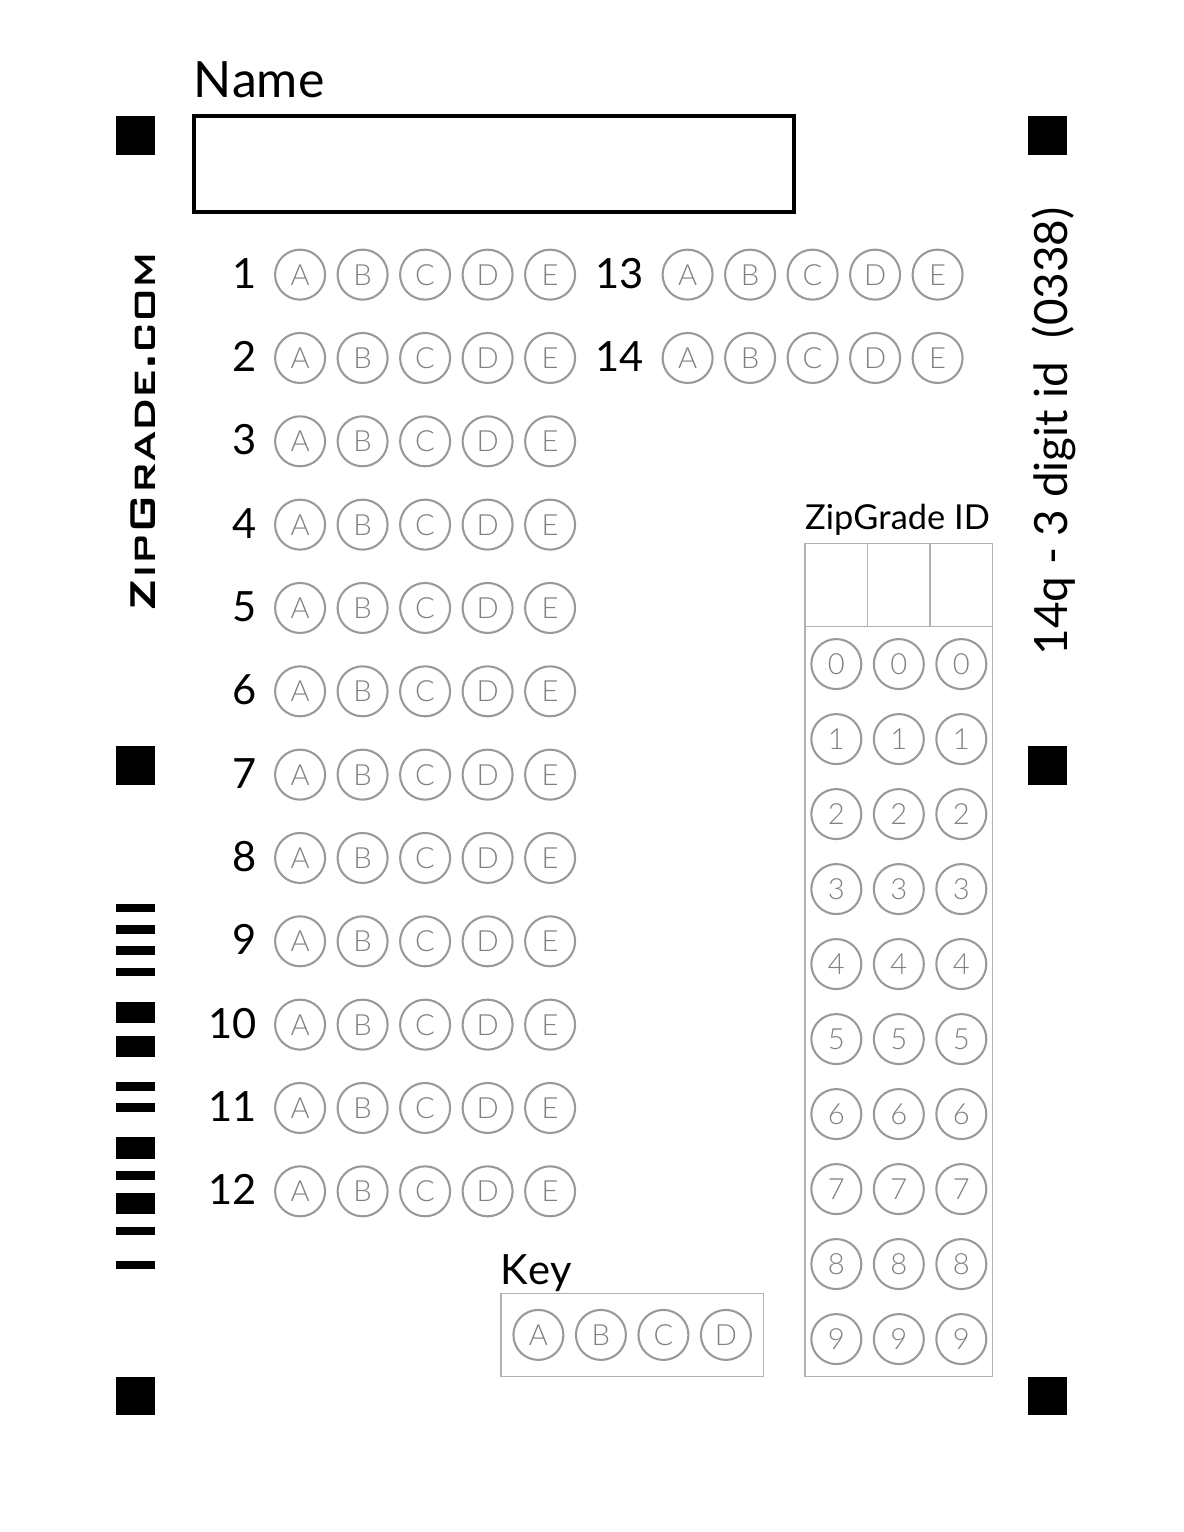
\includegraphics[width=11.55cm]{14Q.png}};
    \fill (#1,#2) circle (0.25);
    \node[anchor=west] at (-7.5,14.5) {\Large \bf \sc \mytitle};
  \end{tikzpicture}
\end{flushright}
}



\scantron{5.4}{2.1}
\bottommatter
\topmatter


\pagebreak

\scantron{6}{2.1}
\bottommatter
\topmatter

\pagebreak

\scantron{6.6}{2.1}
\bottommatter
\topmatter

\pagebreak
\scantron{7.2}{2.1}
\bottommatter
\topmatter


\end{document}